\documentclass[a4paper,10pt]{ltjsarticle}

% 各種字体
% cf. http://www.yamamo10.jp/yamamoto/comp/latex/make_doc/formula/amsmath_symbol/index.php
\usepackage{amsmath,amssymb,amsfonts}

% 定番スニペット
% cf. https://mirrors.ctan.org/macros/latex/contrib/physics2/physics2.pdf
\usepackage{physics2}
% automatic braces
\usephysicsmodule{ab}

% 単位
% cf. http://www.yamamo10.jp/yamamoto/comp/latex/make_doc/unit/index.php
\usepackage{siunitx}

% 画像挿入
\usepackage{graphicx}
% ハイパーリンク, URL 挿入
\usepackage{hyperref,url}

% 改ページできるフレーム
\usepackage{framed}
% 色付き文字
\usepackage{xcolor}

%-----------%
% コード関連 %
%-----------%

% 疑似コード
% cf. https://tug.ctan.org/macros/latex/contrib/algorithmicx/algorithmicx.pdf
% cf. https://qiita.com/tomoyk/items/6016123b5c9034bb0087
\usepackage{algorithm}
\usepackage{algpseudocode}

% コードブロック
% cf. https://cloudlatex.io/latex-notation#%E3%82%BD%E3%83%BC%E3%82%B9%E3%82%B3%E3%83%BC%E3%83%89
\usepackage{listings}
% \usepackage{jvlisting}
\lstset{%
  language={C}, % 載せるソースコードの言語を指定する
  basicstyle={\small}, % 通常のソースのフォントを設定
  identifierstyle={\small},% 変数名などのフォントを設定
  commentstyle={\small\itshape\color[rgb]{0,0.5,0}}, % コメントのフォントを設定
  keywordstyle={\small\bfseries\color[rgb]{0,0,1}}, % 予約語のフォントを設定
  ndkeywordstyle={\small}, % keywordstyle以外に定義されている予約語のフォントを設定
  stringstyle={\small\ttfamily\color[rgb]{1,0,1}}, % 文字列のフォントを設定
  frame={tb}, % 実線で描く枠の位置指定
  breaklines=true, % 自動改行の有無
  columns=[l]{fullflexible},% 文字間の余白
  numbers=left, % 行番号の位置
  numberstyle={\scriptsize}, % 行番号のフォント
  stepnumber=1, % 行番号の刻み幅
  lineskip=-0.5ex, % 行間
}

% インラインコードブロック (\lstinline)
% cf. https://tex.stackexchange.com/questions/357227/adding-background-color-to-verb-or-lstinline-command-without-colorbox
\usepackage{xpatch}
\usepackage{realboxes}
\definecolor{mygray}{rgb}{0.95,0.95,0.95}
\makeatletter
\xpretocmd\lstinline{\Colorbox{mygray}\bgroup\appto\lst@DeInit{\egroup}}{}{}
\makeatother

%---------%
% 参考文献 %
%---------%

% cf. https://tex.stackexchange.com/questions/655812/how-to-include-a-url-in-a-customized-way-with-unsrt
\usepackage[numbers, sort]{natbib}
\bibliographystyle{unsrtnat}

%---------------%
% 適宜切り替える %
%---------------%

% 、。と ,. の切り替え (LuaLaTeX 専用)
\usepackage{newunicodechar}
\newunicodechar{、}{,}
\newunicodechar{。}{.}

% ページ数を消す
% \pagestyle{empty}

\begin{document}

\section{サンプル}

\LaTeX。
% 助詞の連続のエラー例
textlint で文法ががェックできます。
% である・ですます のエラー例
本日はは晴天である。
AdS/CFT~\cite{maldacena1999large}
の概要を図~\ref{fig:adscft}に示します。
アルゴリズム体操はアルゴリズム~\ref{alg:excersise}に示します。
インラインのコードブロックは\lstinline|sudo apt update|で書けます。

% 図の例
\begin{figure}[tbp]
  \begin{center}
    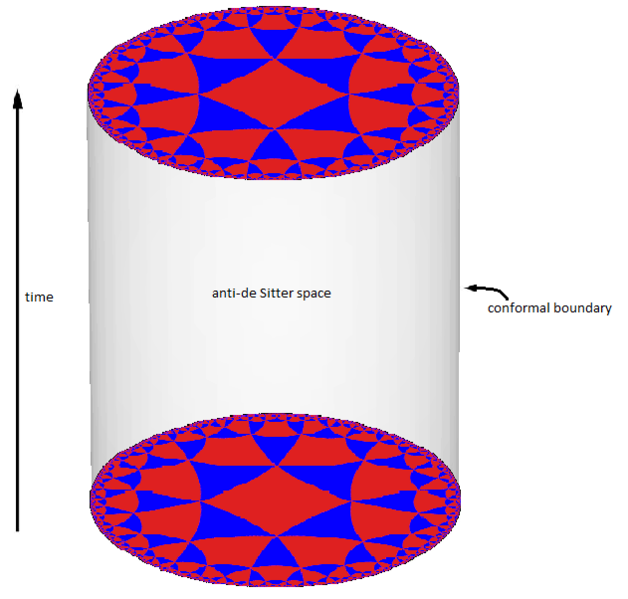
\includegraphics[width=8cm]{img/sample.png}
    \caption{AdS/CFT対応の概念図~\cite{adscftwiki}}
  \end{center}
  \label{fig:adscft}
\end{figure}

% アルゴリズムの例
\begin{figure}[tbp]
  \begin{algorithm}[H]
    \caption{アルゴリズム体操}
    \label{alg:excersise}
    \begin{algorithmic}
      \Function {体操}{}
      \ForAll {こっち, あっち}
      \State {ふたりで まえならえ}
      \EndFor
      \EndFunction
    \end{algorithmic}
  \end{algorithm}
\end{figure}

% ソースコードの例
\begin{lstlisting}[caption=listing,label=listTest]
  #include<stdio.h>
  int main(void){
      printf("Hello World!!");
      return 0;
  }
\end{lstlisting}

\bibliography{reference}

\end{document}